\chapter{Sterren en de nachtelijke hemel}\label{ch:g5:stars-night-sky}

Ver van de stadslampen, op een heldere nacht zonder maan, is de hemel
overvol: duizenden vonkjes, zwak en fel, wit en oranje. Zeelieden
voeren erop, boeren zaaiden ernaar, en elke wetenschap begon met
verwondering erover. Wat zijn het --- en waarom draaien ze zo netjes
boven ons hoofd terwijl wij slapen?

\section{Wat een ster is}

\begin{example}[Ontelbare zonnen]\label{ex:g5:stars-night-sky:suns}
Elke \omterm{def:g4:solar-system:star}{ster} is een zon: een reusachtige bal gloeiend hete stof die haar
eigen \omterm{def:g1:light-and-shadows:source}{licht} uitstort --- veel ervan zijn machtiger dan onze eigen Zon.
Ze zien er om maar één reden uit als nederige vonkjes: afstand. De Zon
is onze \omterm{def:g4:solar-system:star}{ster} van hiernaast; de andere staan zo ver dat zelfs
\omterm{def:g1:light-and-shadows:source}{licht}, de kampioen hardlopen die in geen tijd een kamer oversteekt,
\emph{jaren} onderweg is vanaf de dichtstbijzijnde. De nachtelijke
hemel is een menigte zonnen, door afstand tot geglinster gekrompen.
\end{example}

\begin{omfigure}
\begin{tikzpicture}[scale=0.85]
  \fill[omThm] (1.1,1.4) circle (0.4);
  \foreach \a in {0,45,...,315} {
    \draw[omThm] (1.1,1.4) ++(\a:0.55) -- ++(\a:0.22);
  }
  \node[below, font=\small] at (1.1,0.75) {een lamp dichtbij};
  \fill[omThm] (8.6,1.4) circle (0.07);
  \node[below, font=\small] at (8.6,0.75)
    {dezelfde lamp ver in de straat};
  \node[above, font=\small] at (5.3,2.3)
    {afstand krimpt elk licht tot een vonkje};
\end{tikzpicture}

{\small Eén straatlantaarn, dichtbij en ver weg gezien: de helderheid
zwakt af met de afstand. De sterren zijn lampen op afstanden voorbij
alle wegen.}
\end{omfigure}

\begin{omfigure}
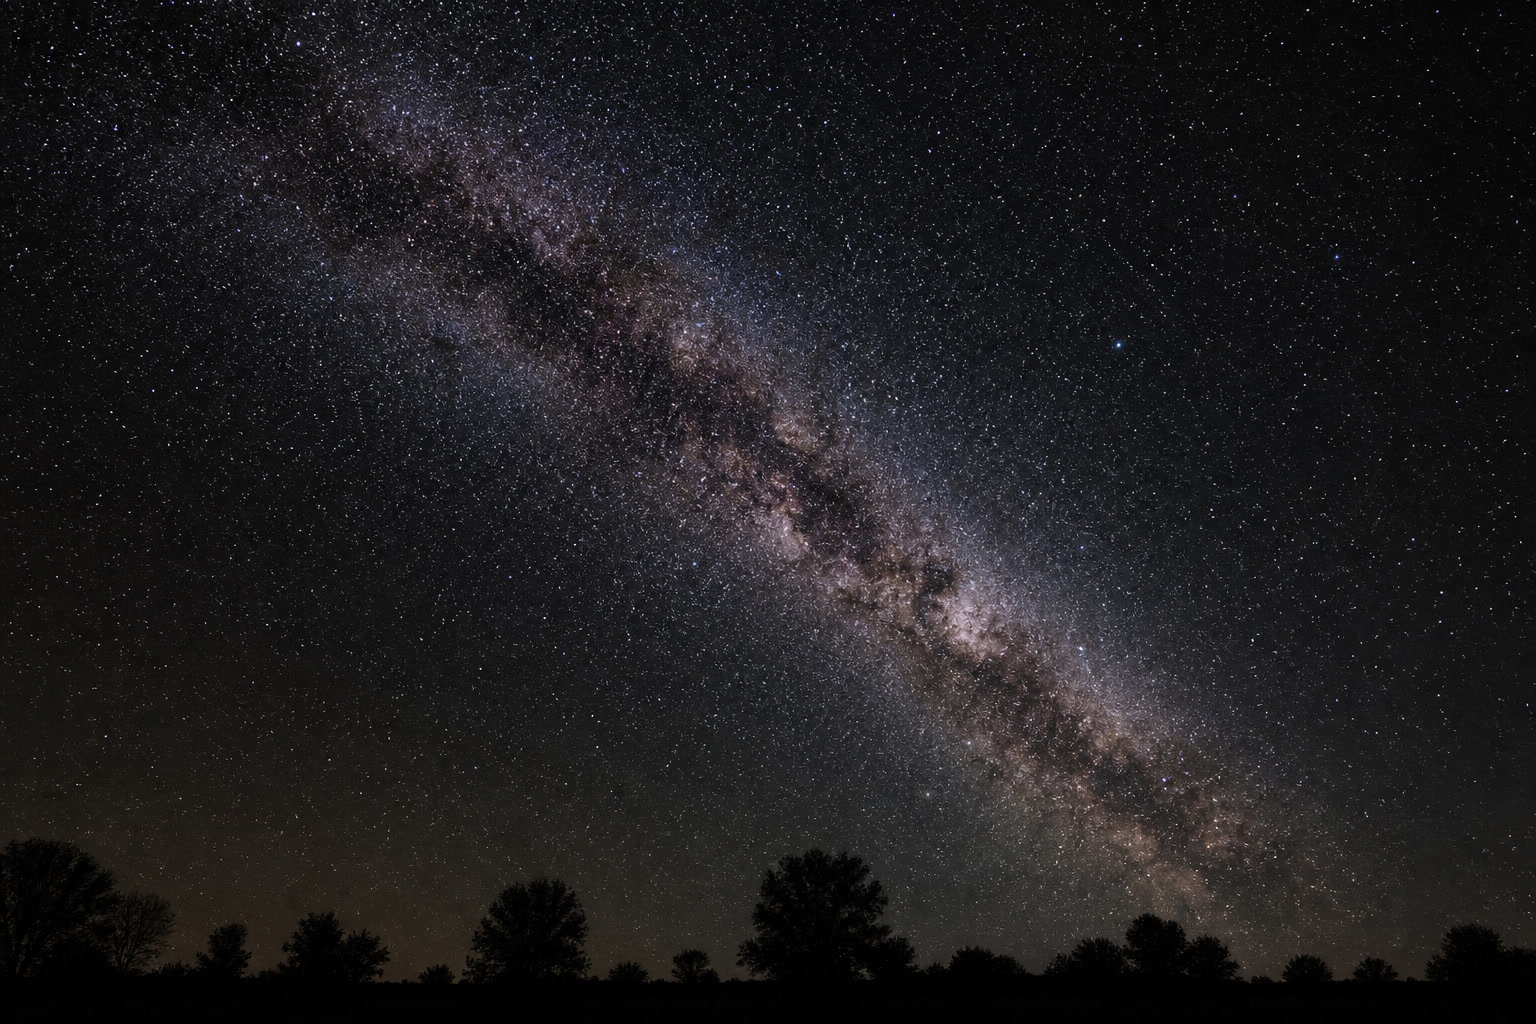
\includegraphics[width=0.58\linewidth]{images/book1/ai/g5-stars-night.jpg}

{\small Een werkelijk donkere nacht ver van de stad: duizenden zonnen, en de zachte band van de \omterm{ex:g5:stars-night-sky:milkyway}{Melkweg} die de hemel doorkruist.}
\end{omfigure}

\begin{example}[Sterrenkleuren]\label{ex:g5:stars-night-sky:colors}
Kijk goed en de vonkjes zijn niet allemaal wit: sommige branden
oranjerood, sommige geel als onze Zon, sommige blauwwit. De kleur is
een boodschap over hitte --- en ze loopt tegengesteld aan kranen en
verfpotten: de oranje sterren zijn de \emph{koelste} van de familie,
en de blauwwitte de heetste, veel heter dan de Zon. Een gloeiende kool
en een witgloeiend stuk staal vertellen hier op Aarde hetzelfde
verhaal: heter gloeit witter.
\end{example}

\begin{remark}[Waar de sterren overdag heen gaan]\label{rem:g5:stars-night-sky:daytime}
De sterren gaan nooit weg. Ze schijnen om twaalf uur 's middags precies
zo boven je als om middernacht --- maar de daghemel is overspoeld met
zonlicht dat door de \omterm{def:g2:air-around-us:air}{lucht} verstrooid wordt, een blauwe felheid die veel
sterker is dan welk vonkje ook. Een kaars is onzichtbaar naast een
vreugdevuur. Zodra de Zon ondergaat en de felheid wegloopt, wordt de
vaste menigte aan de hemel gewoon weer zichtbaar.
\end{remark}

\section{Kaarten van sterren}

\begin{definition}[Sterrenbeeld]\label{def:g5:stars-night-sky:constellation}
Een \emph{sterrenbeeld}\index{sterrenbeeld} is een patroon van heldere
sterren met een naam --- een jager, een zwaan, een grote beer ---
lang geleden bedacht door hemelkijkers als kaart en geheugensteun. De
sterren van een sterrenbeeld zijn in werkelijkheid geen buren; ze
staan alleen op één lijn gezien vanaf de Aarde. Maar de patronen
liggen vast: je grootouders leerden precies dezelfde vormen.
\end{definition}

\begin{method}[De Poolster vinden]\label{met:g5:stars-night-sky:northstar}
De hemel biedt een gratis \omterm{def:g4:magnets-and-compass:compass}{kompas}:
\begin{enumerate}
  \item zoek de Steelpan --- zeven heldere sterren, een steelpan met
        een lange steel, het hele jaar door makkelijk te vinden;
  \item neem de twee sterren aan de voorrand van de pan --- de
        \emph{wijzers};
  \item verleng de lijn van de ene naar de andere, verder over de
        hemel, ongeveer vijf keer hun onderlinge afstand;
  \item de bescheiden \omterm{def:g4:solar-system:star}{ster} waar je uitkomt is de
        \emph{Poolster}\index{Poolster} --- laat er een schietlood van
        omlaag hangen tot de horizon, en daar is het noorden.
\end{enumerate}
Controleer het met je \omterm{def:g4:magnets-and-compass:compass}{kompas}: naald en \omterm{def:g4:solar-system:star}{ster} zijn het eens. Zeelieden
hebben eeuwenlang hun leven op die overeenstemming verwed.
\end{method}

\begin{omfigure}
\begin{tikzpicture}[scale=0.85]
  % the seven stars of the Dipper: handle, then bowl
  \foreach \x/\y in {0.16/3.59, 1.07/3.03, 1.79/2.53, 2.51/2.02,
      1.82/1.32, 2.60/0.60, 3.40/1.28} {
    \fill[omExo] (\x,\y) circle (0.09);
  }
  \draw[thin, omExo] (0.16,3.59) -- (1.07,3.03) -- (1.79,2.53)
    -- (2.51,2.02) -- (1.82,1.32) -- (2.60,0.60) -- (3.40,1.28)
    -- (2.51,2.02);
  % the pointers' line, five spacings out to the North Star
  \draw[dashed, omThm, -Stealth] (3.40,1.28) -- (6.25,3.71);
  \fill[omThm] (6.60,4.00) circle (0.13);
  \node[right, font=\small, omThm] at (6.85,4.00) {Poolster};
  \node[below, font=\small] at (3.1,0.12)
    {de Steelpan, met haar twee wijzersterren};
  \node[right, font=\small] at (5.35,2.15)
    {vijf afstanden langs de lijn van de wijzers};
\end{tikzpicture}

{\small De wegwijzer van de nachtelijke hemel: de twee wijzersterren
van de Steelpan wijzen recht naar de \omterm{met:g5:stars-night-sky:northstar}{Poolster}.}
\end{omfigure}

\section{De draaiende hemel}

\begin{proposition}[De hemel draait om de Poolster]\label{prop:g5:stars-night-sky:wheel}
De hele menigte sterren draait de nacht door langzaam in grote
cirkels over de hemel --- allemaal om één bijna onbeweeglijk punt: de
\omterm{met:g5:stars-night-sky:northstar}{Poolster}. Daarboven beweegt in werkelijkheid niets zo netjes; het is
onze eigen Aarde die draait, zoals ze de Zon over de daghemel laat
trekken. De \omterm{met:g5:stars-night-sky:northstar}{Poolster} verroert zich nauwelijks doordat ze toevallig
bijna precies boven de draaias van de Aarde staat --- de ene richting
die de draaiing met rust laat.
\end{proposition}

\begin{omfigure}
\begin{tikzpicture}[scale=0.85]
  \fill[omThm] (5.5,3.4) circle (0.11);
  \node[above, font=\small] at (5.5,3.6) {Poolster};
  \foreach \r in {0.9, 1.7, 2.5} {
    \draw[omExo, thick] (5.5,3.4) ++(-35:\r) arc (-35:215:\r);
  }
  \foreach \r/\a in {0.9/40, 1.7/130, 2.5/75} {
    \fill[omExo] (5.5,3.4) ++(\a:\r) circle (0.08);
  }
  \draw[thick] (1.5,0.6) -- (9.5,0.6);
  \node[below, font=\small] at (5.5,0.35)
    {horizon --- een nacht met lange sluitertijd, getekend};
\end{tikzpicture}

{\small Richt een camera op de \omterm{met:g5:stars-night-sky:northstar}{Poolster} en laat hem de hele nacht
staren: elke \omterm{def:g4:solar-system:star}{ster} tekent een boog om het stille punt. Het wiel van de
hemel is de draaiing van de Aarde, van binnenuit gezien.}
\end{omfigure}

\begin{example}[Onze stad van sterren]\label{ex:g5:stars-night-sky:milkyway}
Op de donkerste nachten welft een zwakke melkachtige band dwars over
de hemel: de \emph{Melkweg}\index{Melkweg}. Een verrekijker lost de
melk op in de waarheid: ontelbare sterren, te zwak en te dicht opeen
om met het oog te scheiden. Het is onze eigen sterrenstad van
binnenuit gezien --- een plat, wervelend eiland met meer zonnen dan er
zandkorrels op een strand liggen, met onze Zon in een rustige
buitenwijk. Elke \omterm{def:g4:solar-system:star}{ster} die je met het blote oog kunt zien is een buur
uit deze ene stad.
\end{example}

\begin{remark}[Blijf omhoogkijken]\label{rem:g5:stars-night-sky:lookup}
De sterrenkunde is de oudste wetenschap, en de enige waarvan het
laboratorium elke heldere nacht gratis opengaat. Een deken, een donker
plekje weg van de straatlantaarns, en geduld terwijl je ogen wakker
worden in het donker --- dat is de hele uitrustingslijst. De Steelpan,
de \omterm{met:g5:stars-night-sky:northstar}{Poolster}, een \omterm{def:g4:solar-system:planet}{planeet} of twee en de \omterm{ex:g5:stars-night-sky:milkyway}{Melkweg} vormen een mooie
eerste expeditie; de diepere wetten van het \omterm{def:g1:light-and-shadows:source}{licht} van de
sterren zullen je jaren later, tegen het einde van deze cursus, goed
voorbereid aantreffen.
\end{remark}

\section{Oefeningen}

\begin{exercise}[$\star$]\label{exo:g5:stars-night-sky:1}
Wat is een \omterm{def:g4:solar-system:star}{ster}? Waarom zien sterren eruit als piepkleine vonkjes
terwijl veel ervan onze Zon overstralen?
\end{exercise}

\begin{exercise}[$\star$]\label{exo:g5:stars-night-sky:2}
Staan de sterren om twaalf uur 's middags nog aan de hemel? Waarom
kunnen we ze niet zien?
\end{exercise}

\begin{exercise}[$\star$]\label{exo:g5:stars-night-sky:3}
Een oranje \omterm{def:g4:solar-system:star}{ster} en een blauwwitte \omterm{def:g4:solar-system:star}{ster} schijnen naast elkaar. Welke
is heter? Welke alledaagse gloed vertelt hetzelfde kleurenverhaal?
\end{exercise}

\begin{exercise}[$\star$]\label{exo:g5:stars-night-sky:4}
Wat is een \omterm{def:g5:stars-night-sky:constellation}{sterrenbeeld}? Staan zijn sterren werkelijk dicht bij
elkaar?
\end{exercise}

\begin{exercise}[$\star$]\label{exo:g5:stars-night-sky:5}
Beschrijf stap voor stap hoe je vanaf de Steelpan de \omterm{met:g5:stars-night-sky:northstar}{Poolster} vindt.
\end{exercise}

\begin{exercise}[$\star$]\label{exo:g5:stars-night-sky:6}
Wat is er bijzonder aan de plaats van de \omterm{met:g5:stars-night-sky:northstar}{Poolster} aan de draaiende
hemel, en welk alledaags instrument vervangt ze?
\end{exercise}

\begin{exercise}[$\star$]\label{exo:g5:stars-night-sky:7}
De sterren draaien 's nachts in nette cirkels over de hemel. Wat
draait er in werkelijkheid? Wat laat diezelfde draaiing nog meer over
de daghemel paraderen?
\end{exercise}

\begin{exercise}[$\star$]\label{exo:g5:stars-night-sky:8}
Wat blijkt de melkachtige band over de donkerste hemel te zijn als je
er met een verrekijker naar kijkt? Wat is hij werkelijk?
\end{exercise}

\begin{exercise}[$\star\star$]\label{exo:g5:stars-night-sky:9}
Een camera die je de hele nacht op de \omterm{met:g5:stars-night-sky:northstar}{Poolster} gericht laat staan
legt cirkels vast; gericht op de oostelijke horizon legt hij juist
opstijgende schuine strepen vast. Verklaar beide foto's met één
draaiende Aarde.
\end{exercise}

\begin{exercise}[$\star\star$]\label{exo:g5:stars-night-sky:10}
Een schipbreukelinge heeft op een heldere nacht geen \omterm{def:g4:magnets-and-compass:compass}{kompas}, geen
telefoon --- en geen haast. Leg uit hoe de hemel haar zowel een
richting als, met geduld, een klok aanreikt. (Twee ideeën uit het
hoofdstuk, één draaiende hemel.)
\end{exercise}

\begin{exercise}[$\star\star$]\label{exo:g5:stars-night-sky:11}
Het \omterm{def:g1:light-and-shadows:source}{licht} van een verre \omterm{def:g4:solar-system:star}{ster} is jaren onderweg naar jouw oog. Zie
je die \omterm{def:g4:solar-system:star}{ster} vanavond zoals ze \emph{nu} is? Waar kijk je eigenlijk naar
--- en waarom maakt dat van elke telescoop een soort tijdmachine?
\end{exercise}
